\documentclass{article}
\usepackage{graphicx}

\begin{document} 
\begin{center}
{\bf \Large  Homework 1} \\
(Due on: Wed, October 10 by 8:00PM via e-mail)
\end{center}

\noindent  The aim of this homework is to introduce you to feedback control systems and for you to use your MATLAB and SIMULINK skills in the context of a simulation of a feedback control system. The control system in Fig. 1. is in detail covered in the class and presented in my lecture notes with all the parameters. \\

\begin{figure}[h]
\begin{center}
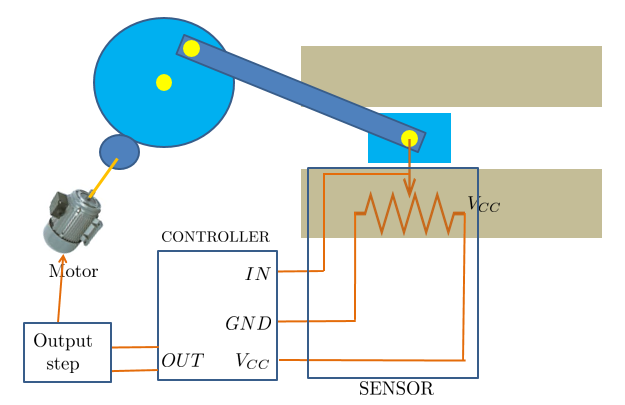
\includegraphics[width=0.5\textwidth]{Fig1.png}
\end{center}
\vspace{-0.6cm}
\caption{}
\end{figure}

\noindent a) Explain why in the feedback loop presented in the lecture notes we cannot use negative values for $K_p$ and what the benefit of a large positive $K_p$ value is. \\

\noindent b) Run the simulation {\bf CE141IntroModel1.mdl} for input values $1$, $2$, $3$,... and find the highest integer value $u_{max}$ (for which the motor does not work). Can you explain (in words) the trend in the frequency of $x_2$ plots and check if the maximal and minimal values of $x_2$ correspond to those in the lecture notes? \\

\noindent c) The simulink model {\bf CE141IntroModel2.mdl} includes
both the system and the proportional controller $K_p$. The reference
for the controller changes as a square pulse from 4 to 5.4 with a period of 10s and a duty cycle of 50\%. Find the largest value of the gain $K_p$ for which the control $u$ value does not exceed $u_{max}$ from (b). How does the limit on $u$ impact the performance of the feedback control loop? \\

\noindent d) Use $K_p$ from (c) and adjust the model in such a way that the reference changes from 4.2 to 4.8. Include the figures in your report.  \\

\noindent e) The simulink model {\bf CE141IntroModel3.mdl} 
models the system controlled by a digital proportional controller. 
Go back and forth between the simulation results of this model 
and of the one in {\bf CE141IntroModel2.mdl} until you find 
the value of $K_p$ that in both simulations results in a similar 
position ($x_2$) and control ($u$) signals. Include the figures 
in your report.  \\

\noindent {\bf Note }: You are free to use any part of the code provided with this homework. Please try to understand the code.

\end{document}